\chapter{System Overview}
\label{ch:system}

Broadly speaking, we are aiming to develop a suite of open-source technologies
for artificial social intelligence. For ASIST Study 3, we are particularly
interested in studying team coordination and communication.

For ASIST Study 3, we will deploy five containerized components. Four of them
can be classified as `analytical components' (ACs) in the parlance of the ASIST
program, and one as an `ASI', i.e. an AI agent imbued with artificial social
intelligence and designed to provide helpful interventions. In principle, the
four ACs could be bundled and deployed as part of our ASI, but we opt to keep
them separate as we expect that the resulting modularity will be beneficial for
future applications and results in additional system robustness.


\section{Analytical Components}

We list the analytical components we are deploying for ASIST Study 3 in
\autoref{tab:study_3_acs}. The system architecture into which they fit is shown
in \autoref{fig:nlp-architecture}.

\begin{table}
    \small
    \begin{tabularx}{5.5in}{llXl}
        \toprule
        Component           & Inputs                        & Outputs               & Chapter\\\midrule
        ASR Agent           & Raw audio                     & Transcriptions, word-level timings     & \\
        SpeechAnalyzer      & Raw audio, transcriptions     & Sentiment and personality trait labels & \autoref{ch:sentiment_analysis}\\
        DialogAgent         & Transcriptions, chat messages & Structured events                      & \autoref{ch:rule_based_ie}\\
        DialogActClassifier & Transcriptions                & Dialog act labels                      & \autoref{ch:da_classification}\\
        \bottomrule
    \end{tabularx}
    \caption{%
        Analytical components we are deploying for ASIST Study 3, along with
        their inputs, outputs, and correspnding sections in this document that
        describe their capability in greater detail.
    }
    \label{tab:study_3_acs}
\end{table}


\begin{figure}
    \centering
    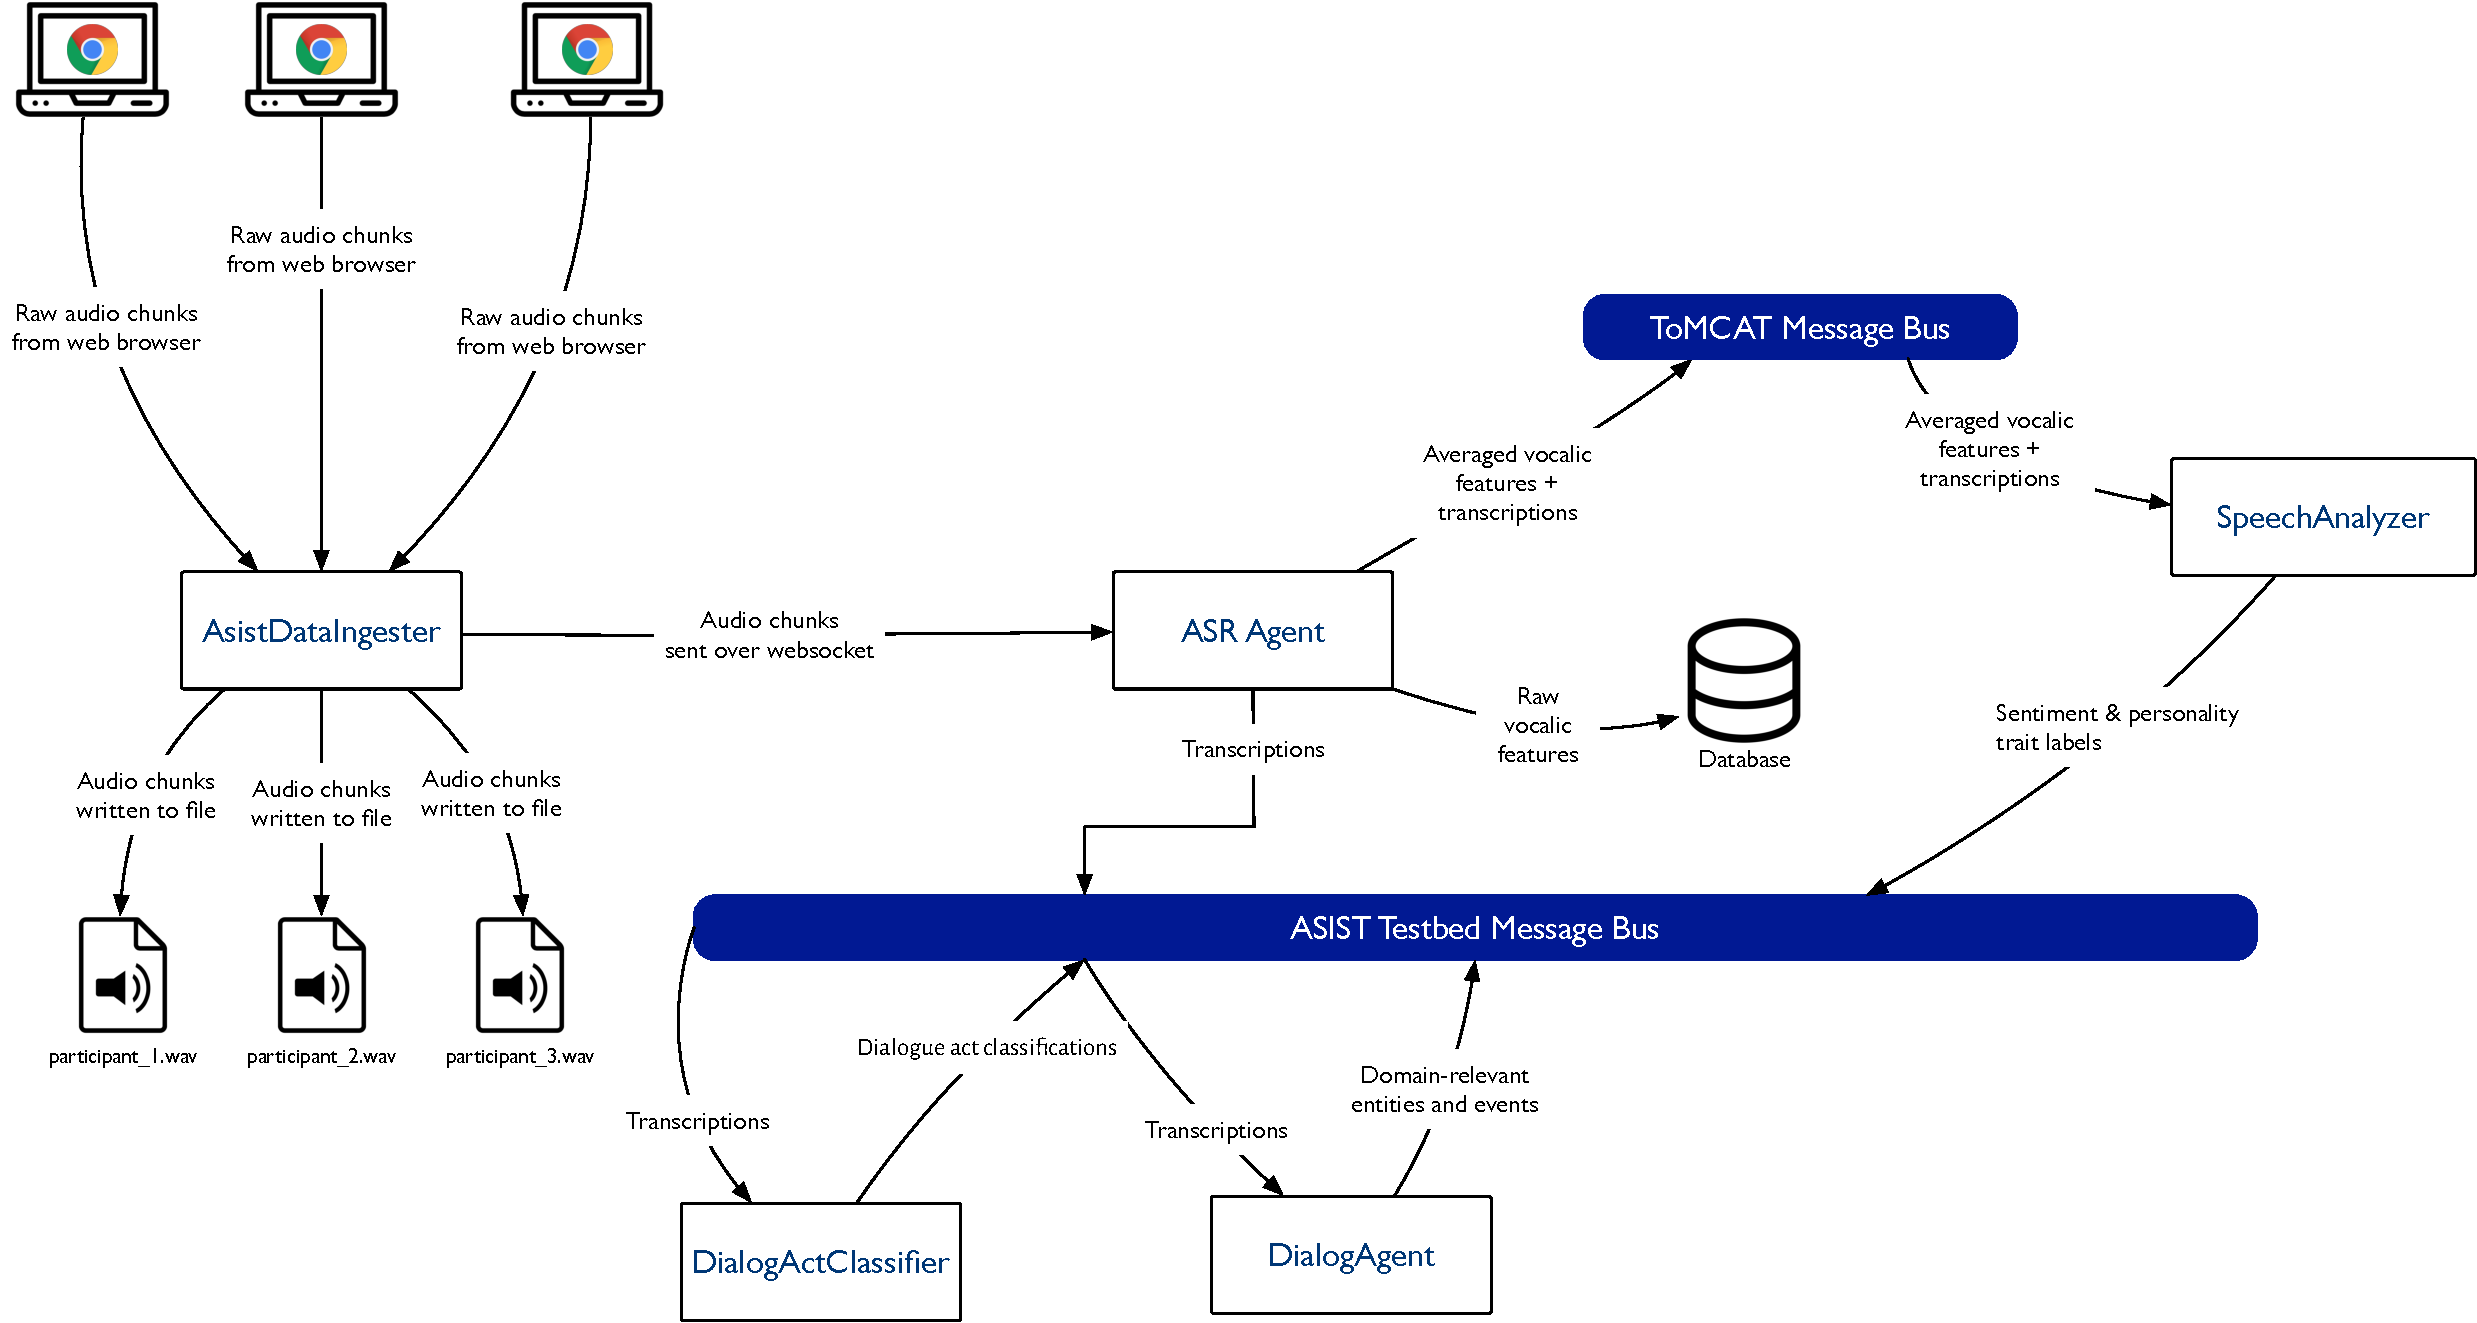
\includegraphics[width=4in]{images/nlp_architecture}
    \caption{Architecture of our multi-participant dialogue analysis system.}
    \label{fig:nlp-architecture}
\end{figure}

\section{Artificial Social Intelligence}

The outputs of the aforementioned analytical components are among the inputs to
our artificial social intelligence agent, ToMCAT. The core capabilities and
planned interventions of our agent are described in \autoref{ch:pgm}.
